
\section{Evaluation}
\label{sec:eval}

\subsection{Experimental setup}
\label{sec:eval:setup}

\edb{TO FIXUP once we decide final location.   Current values are for EPFL} 

Our experimental setup consists of a cluster of 19 clients and one
server connected by an XXX low-latency 10GbE switch.  The client
machines are dual Xenon XXX running at XXX Ghz with a single, Intel
XXX 10GbE NIC connecting to the switch.  The server is a dual-Xeon XXX
running at XXX Ghz with XXX GB of DRAM with four Intel XXX NICs.  Each
socket (client or server) has 8 cores and 16 hyperthreads.  When
reporting multi-core scalability, we report results with
hyperthreading enabled, and both hyperthreads of the cores are used.

The server is connected to
the switch via a 4x10GbE bond configured in as a L2+L3
hash~\cite{missing} in the switch via LACP~\cite{ieee802.3ad}.  Jumbo
frames are never enabled.  Our baseline configuration in each machine
is the Ubuntu XXX distribution running the XXX Linux kernel.  Although
the server has two sockets, our experiments pin IRQs, processes, and
the IX dataplane onto a single socket and use memory from that socket;
all NICs are attached to that socket via the PCIe root complex.

\christos{We should organize the eval in the following way: first
  micro-benchmarks that showcase each of the advantages (high packet
  rate, low latency/jitter, high connection/churn). The title of the
  subsection should indicate the aspect evaluated. Then there should
  a subsection on full app eval (memcache hopefully).}

\subsection{Ping-Pong (NetPIPE)}

\begin{figure}
\begin{centering}
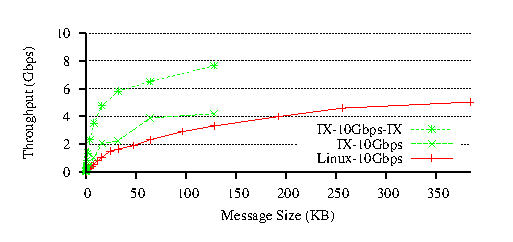
\includegraphics{figs/pingpong.eps}
\caption{NetPIPE performance for varying message sizes and system software configurations.}
\label{fig:pingpong}
\end{centering}
\end{figure}



%%%
%%%  use the ping-pong test to measure the half rountrip latency @ 64B
%%% 

\begin{table}[b]
\vspace{-1em}
\begin{center}
\begin{small}
\begin{tabular}{|l|c|c|}
\hline
Workload &  Avg lat. & 99\% lat. \\
\hline
Linux(base)-Linux(base)  & 60\microsecond & 0\microsecond\\
Linux(opt)-Linux(opt)    & 0\microsecond &  0\microsecond \\
mTCP-mTCP                & 0\microsecond &  0\microsecond \\
Linux(opt)-\ix           & 0\microsecond &  38\microsecond\\
\ix-\ix                  & 0\microsecond &  0\microsecond\\
\hline
\end{tabular}
\caption{Netpipe half-roundtrip latency (s=64B)}
\vspace*{-2em}
\label{tbl:pingpong}
\end{small}
\end{center}
\end{table}



Fig.~\ref{fig:pingpong} illustrates the importance of system software
design and configuration tradeoffs using the NetPIPE ping-pong
benchmark~\cite{snell1996netpipe} that exchanges a fixed-size message
between two servers.  Although the application is trivial, it provides
a good proxy for the effective performance of synchronous remote
procedure calls in uncontended situations.  We compare the performance
of (i) an out-of-the-box Ubuntu XXX configuration
(\texttt{Linux-base}) running an unmodified NetPIPE v3.7.2; (ii) a
tuned configuration of the same kernel (\texttt{Linux-opt})) with the
same application; (iii) between two mTCP-based equivalent
applications; (iv) a hybrid version in which a Linux client talking to
an \ix server; and finally (v) between two \ix systems.  For the same
application and hardware configuration (described in
\S\ref{sec:eval:setup}), the differences are dramatic.  We see that
\ix-\ix achieves 50\% of the asymptotic bandwdith with messages as small
as \george{XXX bytes}.  In constrast, both Linux configurations remain
latency-bound.  Although mTCP, ....


Table~\ref{tbl:pingping} lists the average and 99\% percentile half
round-trip latencies for small messages (64B), using the same netpipe
benchmark.  \edb{TODO - COMMENTARY.}

\subsection{Handling short TCP transactions}


%% put the key last to have correct numbering

\begin{figure*}[t]

\centering
  \vspace*{0.3in}
 \subfloat[Multi-core scalability (n=1;s=64B)]{
  \label{fig:short:mcore}
   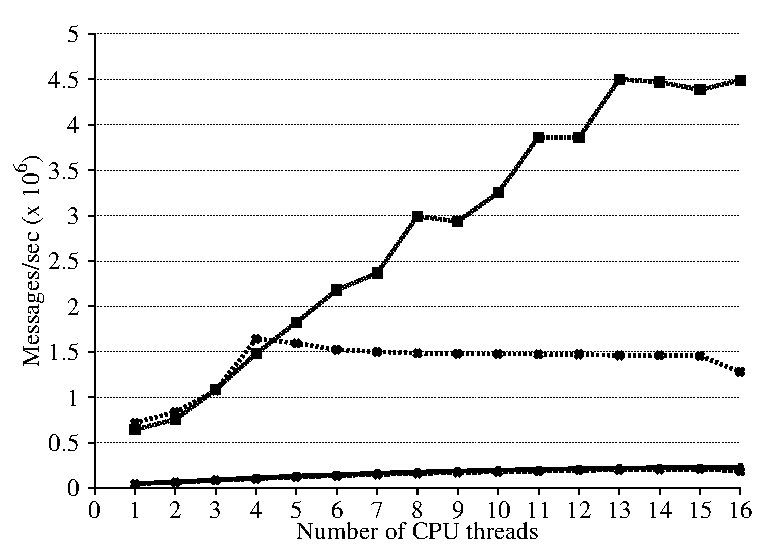
\includegraphics{figs/short-mcore.eps}}
 \hspace{.01in}
 \subfloat[$n$ roundtrips per conn. (core=8,s=64B)]{
  \label{fig:short:roundtrips}
  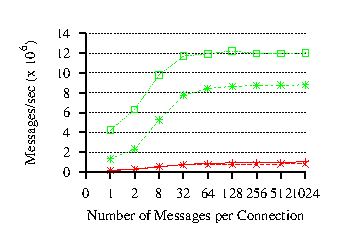
\includegraphics{figs/short-roundtrips.eps}}
  \hspace{.01in}
 \subfloat[Different message sizes $s$ (core=8,n=1)]{
  \label{fig:short:size}
  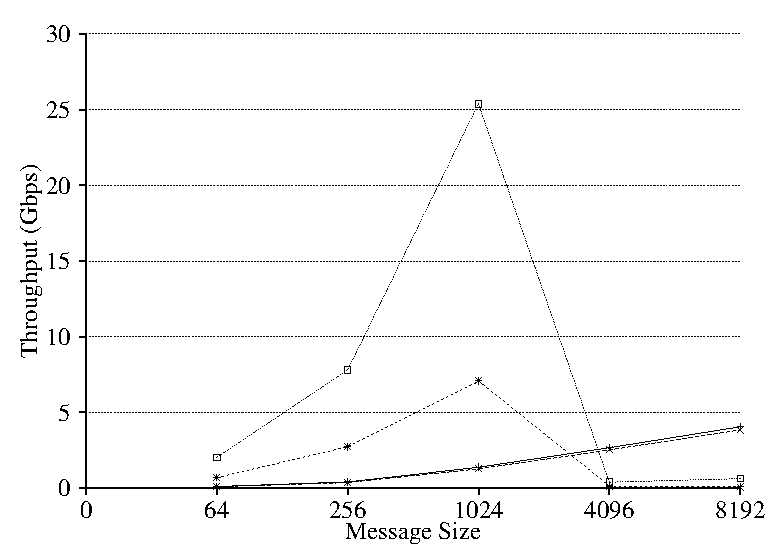
\includegraphics{figs/short-size.eps}}
 \centering
  \vspace{-1.9in}
  \subfloat{
\includegraphics{figs/short-key.eps}}
 \vspace{1.5in}
 \
\caption{Short message performance.}
 \label{fig:short}

\end{figure*}


We first evaluate \ix's scalability with a benchmark that stresses
connection churn in server, as used to evaluate
Megapipe~\cite{han2012megapipe} and mTCP~\cite{jeong2014mtcp}:
multiple clients connect to a single server listeningo on a single
port, send a request of size $s$ and wait for an echo of a message of
the same size.  As with netpipe, while accepting the message, the server holds off its
echo response until the message has been entirely received.
Each client performs this synchronous remote procedure
call $n$ times, and then close the connection using a reset
(\texttt{TCP RST}).

Fig.~\ref{fig:short} shows the results. XXX


subsection{Connection Scalability}



%FIXME if different keys


\begin{figure*}[t]

\centering
  \vspace*{0.3in}
 \subfloat[Throughput for varying established connections]{
  \label{fig:connscaling:throughput}
   
\includegraphics[width=.49\textwidth,clip]{figs/blank.eps}}
 \hspace{.02in}
 \subfloat[Avg. and 99\% latency for varying established connections]{
  \label{fig:connscaling:lat}
  
\includegraphics[width=.49\textwidth,clip]{figs/blank.eps}}
\centering
  \vspace{-2.8in}
  \subfloat{
\includegraphics[width=1\textwidth,clip]{figs/short-key.eps}}
 \vspace{2.3in}
 \
\caption{Connection scaling}
 \label{fig:connscaling}

\end{figure*}


We then evaluate \ix's scalabilty when handling a large number of concurrent connections. 

XXX


\subsection{TODO}

\todo Compare apples-to-apples with Megapipe, and mTCP in terms of microbenchmarks.

\todo Baseline comparison of state-of-the art systems include:  Linux (some recent version, with SO\_REUSEPORT); Megapipe (if possible), mTCP (if possible). 

\todo Microbenchmark: short TCP transactions (echo server, as defined in megapipe).   Goal is to beat mTCP (and therefore all others) hands down.

\todo Benchmark: memcached - compare with FB results (?)

\todo Benchmark: lightttpd -- used by Affinity-Accept and mTCP.  

\todo ngnx: an actually used webserver.

